%\documentclass[conference]{IEEEtran}
\documentclass[10pt,conference]{IEEEtran}
\IEEEoverridecommandlockouts
% The preceding line is only needed to identify funding in the first footnote. If that is unneeded, please comment it out.
\usepackage{cite}
\usepackage{amsmath,amssymb,amsfonts}
\usepackage{algorithmic}
\usepackage{graphicx}
\usepackage{textcomp}
\usepackage{xcolor}
\usepackage{url}
\usepackage{listings}
\usepackage{courier}
\usepackage{xspace}
\usepackage{multirow}
\usepackage{colortbl}
\usepackage{blindtext}
\usepackage{float}
\usepackage[font=scriptsize]{caption}
\usepackage[sort&compress,square,comma,authoryear]{natbib}
%\newcommand{\sd}[1]{\textbf{"\textsc{SD:}} \textit{#1}"}

\newcommand{\nnbb}[2]{
    \fbox{\bfseries\sffamily\scriptsize#1}
    {\sf\small$\blacktriangleright$\textit{#2}$\blacktriangleleft$}
   }
\newcommand{\sd}[1]{\nnbb{\textcolor{orange}{St\'{e}f}}{\textcolor{orange}{#1}\xspace}}
\newcommand{\hr}[1]{\nnbb{Henrique}{#1\xspace}}
\newcommand{\ap}[1]{\nnbb{\textcolor{blue}{Apierr}}{\textcolor{blue}{#1}\xspace}}
\newcommand{\Miner}[0]{Miner\xspace}
\newcommand{\Miners}[0]{Miners\xspace}
\newcommand{\miner}[0]{miner\xspace}
\newcommand{\miners}[0]{miners\xspace}
\newcommand{\gas}[0]{gas\xspace}
\newcommand{\Gas}[0]{Gas\xspace}
\newcommand{\Transaction}[0]{Transaction\xspace}

\newcommand{\SmartGas }[0]{\textsc{SmartGas}\xspace}

\newcommand{\eg}{\emph{e.g.,}\xspace}
\newcommand{\ie}{\emph{i.e.,}\xspace}
\newcommand{\etal}{\emph{et al.,}\xspace}
\newcommand{\ct}[1]{{\textsf{#1}}\xspace}
\usepackage[scaled=0.85]{helvet}

\def\BibTeX{{\rm B\kern-.05em{\sc i\kern-.025em b}\kern-.08em
    T\kern-.1667em\lower.7ex\hbox{E}\kern-.125emX}}
\begin{document}

\title{Improving practices in a medium french  company: First step}
% \title{Toward  maintainance of  a commencial software: Time serie model of defects }
%\thanks{Identify applicable funding agency here. If none, delete this.}}

\author{\IEEEauthorblockN{HOUEKPETODJI Mahugnon Honore\IEEEauthorrefmark{1}\IEEEauthorrefmark{2},
Nicolas Anquetil\IEEEauthorrefmark{3}}
\IEEEauthorblockA{\IEEEauthorrefmark{1}University of Lille, France}
\IEEEauthorblockA{\IEEEauthorrefmark{2}Inria Lille - Nord Europe, France}
homahugnon@gmail.com, nicolas.anquetil@inria.fr}


\maketitle

\begin{abstract}
Legacy systems are old software that still does useful tasks.
In industrial software companies, legacy systems are often crucial for the company business model and represent a long-term business investment.
Legacy systems are known to be hard to maintain.
This is the case in a french company whose main product is twenty years old software written in PowerBuilder.
Our long-term goal is to help it re-engineer this system.
But how to validate our intervention?
Little data is available on the system and specifically, past versions of the source code are not easy to recover.
This constrained us on the metrics we could use.
%We evaluate the maintenance state of the system and produce a dashboard to monitor our future actions.
In this paper, we present a lightweight model to characterize the situation of the system and allow us to monitor it in the future.
\end{abstract}

\begin{IEEEkeywords}
Legacy system, software quality model .
\end{IEEEkeywords}

\section{Introduction}
%-------------------------------------------------------------------------------

%Software companies usually invest time and energy to improve the quality of the software they develop to respond to the rising market demands.
Software companies have little spare resources to allocate to software quality improvement or code defect removal.
As a result, they often develop features in a hurry.
As the system grows, it becomes harder and harder to maintain.
%Rewriting this software require time and a lot of resources.
To ensure the future of the system, and through it, of the company itself, some re-engineering actions might be necessary.
The long period of growth and evolution of the systems as well as staff evolution, lead to problems such as dead code, duplicate code, and obsolete documentation. 
The developers at the origin of the application are no longer present, so a large part of the knowledge (and this at different levels of granularity) is scattered or lost. 

This is the situation at CIM, a medium French company, which main business product we are studying.
The system is written in an old language (PowerBuilder) typically unknown to young programmers which translates in a difficulty to hire new developers.
There is also a sense in the development team that the system suffers from architecture erosion and is difficult to maintain or evolve which translates into a steep learning curve for new developers.
We are trying to help this company improve its software engineering practices and restructure the system to improve the situation.


In this paper, we are trying to answer the following question:
How to validate our intervention and can we measure its concrete impact on the system and its evolution?

%How to provides a report on the state of the system to the entire company?
For the reasons explained above, we cannot completely rely on current developers knowledge of the system.
The only usable information about the system is its non-versioned source code and a ticket database.
Past literature often relied on historical data on the source code, for example
cyclomatic complexity \cite{gill91}, or number of lines of code \cite{port18}.
In lack of a reliable software versioning system, we could not use these solutions.


We mine and analyse the ticket database to overcome our problem.
This paper presents the results of this work.

 This paper is structured as follows: we start with related work in section \ref{sec:related-work}, followed by the section \ref{sec:background} in which we present tickets database mining background. 
 In the section \ref{sec:methodology} we present our methodology and conclude in section \ref{sec:conclusion}.
 
\section{Related Work}
%-------------------------------------------------------------------------------
\label{sec:related-work}
Recently, research on mining software repositories has received much attention as it attempts to understand software evolution \cite{Zhan10a}.
Software defect history and source code history are often used to monitor software maintenance or predict the system's quality. 
For instance, software defect prediction using software repositories has already been extensively discussed in the literature as witnessed by many literature surveys: \cite{Catal09,Hall12,Hoss17,Li19a,malh15}.
%"intro": de quoi on va parler et pourquoi en parler ?

%A software defect is a mistake at coding level, which manifests in a deviation from expected behavior. 
%Mining a software defect history helps to collect valuable information about the software life evolution. 
%Software re-engineering monitoring should be supported by prediction models that predict the quality under control (\cite{Lenar17}). 

%Software defect history can be used alone to build a software defect model using statistical techniques or machine learning algorithms to predict post-release defects in software.
But these solutions rely on the availability of source code history. 
For example, \cite{gill91} used McCabe’s cyclomatic complexity metric divided by the size of the system to predict software maintenance productivity.
\cite{port18,Zhan10a} used software defect history and source code history to assess a system evolution to monitor maintenance. 

In our case, the source code history is not easily available as the company does not make use of a version control system.
Thus, we cannot use the methods presented above.

\cite{Herz13a} propose to consider ticket database.
He reports that $33.8\%$ of the bugs studied among five open-source projects were misclassified.
For this reason, other researchers try to automatically re-classify maintenance activities (e.g. \cite{Mock20a,Levin19a}).
 
%Other researchers considered ticket database to characterize a system. For instance, \cite{Levin19a} 
At CIM, maintenance activities classification is more reliable because it drives the entire software evolution process.
We rely on this classification to make our analysis.

We develop a lightweight technique to analyse the ticket database.

%"conclusion": (1) on ne veut pas faire de prediction (2) on n'a pas d'historique de code
%donc: on develop notre propre analyse sur la ticket db.

\section{Study background}
%-------------------------------------------------------------------------------
\label{sec:background}

In this paper, we are interested in characterising the system and its evolution to better evaluate the possible future impact of our intervention. 

\subsection{Presentation of the system studied}
%-------------------------------------------------------------------------------

Legacy systems have a lifespan of several decades, decisions made at the beginning of development and their evolution over the life of the software are often lost. 
This is the case of the system we are studying which is more than 20 years old. 
It is written in Powerbuilder.
Powerbuilder is a programming language and integrated development environment initially developed by PowerSoft. The first version was published in 1992.
Powerbuilder application components are grouped in libraries. 
A Powerbuilder library contains differents type of objects: datawindow, user object, global function, menu, etc. 
Powerbuilder is a procedural language that evolved to (partial) object-orientedness: inheritance and object-oriented features are limited to some object types (windows, user objects and menus). 

The system has 3 MLOC, in 117 Powerbuilder libraries.
The largest library is over 300 KLOC.
The development team varied over time but counts 15 people at the moment, without the testing team which is external to development.

PowerBuilder version supports version control only since its 2017 version, and even this supports is still not entirely satisfying, for example
conflict resolution is performed automatically by the system by choosing one version over the other without asking the developer.
For these reasons, version control management was never used on the system studied.% and the support is not stable. 
However some old major versions or archived in separate directories.
Versions before 2012 are completely lost.
Some version control is done informally inside the team.
When developers work on the same version of the system, they chat with each other to notify which part they are modifying so that others won't modify the same part.
Also, each developer has to write a comment in the source code with his/her name and the date the modification he/she performed. 
%We believe that writing author in a comment in the source can be easily handled by a version control system.


\subsection{Ticket}
%-------------------------------------------------------------------------------
% depuis quand ?
% tres important car utilise dans toute la boite: affectatin du travail, workflow, facturation

At CIM, tickets are stored in the tickets database since 2000.
A ticket represents a unit work.
The ticket database drives the entire software evolution process: assignment of work to developers, management of the workflow to answer a client request, billing information about each task.
There are tickets for fixing defects, writing documentation, adding new features, etc. 
As a consequence, we can rely on a ticket's classification because it is reviewed by the team manager to ensure that it is properly handled.

At CIM, a ticket includes the following characteristics among other things:


At CIM, a ticket includes the following characteristics among other things:

\begin{itemize}
\item the creation date
\item the closing date
\item the estimation of the time needed by the developer to work on the ticket
\item time spent by a developer
  \begin{itemize}
  \item time to analyze
  \item time to implement solution
  \item time to test
  \end{itemize}
  \item the library(ies) impacted
\end{itemize}

\section{Methodology}
%-------------------------------------------------------------------------------
\label{sec:methodology}


Our long-term goal is to help developers re-engineer the system at a small cost.
This is needed to improve the general quality and make future evolution easier, but it needs to be cheap to convince upper management investing in this purely technical task.

Therefore, we need to validate our intervention as well as the restructuring work developers might engage in the future.

\subsection{Souce code versionning}
%-------------------------------------------------------------------------------

Our first action was to introduce a version management system.
We chose Subversion (SVN) because it was simpler to explain to developers that were not familiar with the concepts of version management.
We gave a short training session to the developers, and they are now starting to use it as part of the new process.

Besides, we are reconstructing a summarized source history in SVN by importing one after the other the different major versions currently stored in directories (versions 2012 to 2019). 
We hope that this will help us analyze the system's historical code changes to have additional information about the system evolution.

\subsection{Ticket data analysis}
%-------------------------------------------------------------------------------

Our goal was to characterize the system to be able to measure our impact and that of the developers in the future.
The problem was to extract information from the system that was relevant for the company and for which we could hope to have some impact.
All this within the very restricted context described above.


We turned to the ticket database and elected the following questions:
\begin{itemize}
 \item What is the proportion of evolution versus correction tickets?
 \item How long does it take to close a ticket?
 \item Development time spent on a ticket?
 \item Testing time spent by the developer on a ticket?
 \item Testing time spent by the tester (other teams) on a ticket?
 \item Difference between the time estimated and the actual time for a ticket?
 \end{itemize}
 
%a revoir

The ticket database first needed some cleaning:
\begin{itemize}
  \item Tickets may concern several software systems in the company and different development teams.
  We thus selected tickets related to the system we are studying.
  
  \item The ticket database contains data from 1998  until today. 
  Before 2004, tickets information are not always consistent, for example, missing creation date or missing/incorrect category.
  This constrained us to eliminate tickets prior to 2004.

  \item Up to recently, the name of the library concerned by a ticket was filled manually (free text).
  As a consequence, there are some typos in the names that need to be corrected.
  A simple and frequent case is two swapped characters \emph{cwm\_liq\_ou} instead of \emph{cwm\_liq\_uo} (``uo'' PowerBuilder User Object).
  Some more complex cases require an understanding of the application domain and the system, for example, \emph{uo\_liq} instead of \emph{cwm\_liq\_uo}.
  We identified all the errors manually and corrected them.
  
  \item The category of the ticket is fine-grained whereas we are only interested in evolution versus corrective tickets.
  In our analysis, we recategorize the tickets according to some simple dictionary provided by the team manager.
  
\end{itemize}
 
For all the time questions, the tickets are grouped by month of creation and their value (for example time to close the ticket) are averaged for the month of creation.  
We compute the data for our questions as follows:
\begin{itemize}
  \item We compute the \emph{closing time} of a ticket simply as the time between creation and closing of each (closed) ticket.
\item  The time spent by the developers to implement ist's solution for a ticket is provided in this format: \emph{//number of days//number of hours//number of minute//}.
 We convert this format into duration for each tickets. 
 \item When a developer finishes a development related to a ticket, he tests his solution.  
 The testing time is recorded in the ticket database in the format \emph{//number of days//number of hours//number of minute//}.
  We convert this information in duration and plotted it.
 \item For a ticket, the team manager estimates the time needed to finish the task related to the ticket.
 This estimation is based on the experience of the team manager.  
 We plotted the difference  between the time spent by the developer and the estimation per month over the life cycle of the system.  
 This is to assess if the developer has enough time to develop quality source code.
 %autre metric
\end{itemize}

We then plotted the data simply on a 2 dimension graph, but we noticed a very large variation of the results (nonstationary results) that made it hard to interpret the graphs.
To get smoother plots, we computed the moving average of [month-2; month+2] for each month.
Therefore, plotted data for July 2010 of any time metric correspond to the average time of all tickets opened between May 2010 (inclusive) and September 2010 (inclusive).

Finally, to get a better notion of the trend, we will also plot the linear regression of the curve for each graph.

\subsection{Results}
%-------------------------------------------------------------------------------

\subsection{Souce code versionning}
%-------------------------------------------------------------------------------

The introduction of SVN only started one month ago and we do not have yet significant results to report. 

For the reconstruction of the summarized source history, we already imported major versions until 2015 in a separated repository. 
 %We then grouped them by major release. 
 %We create an SVN repository in which we create a branch for each major release. We are pushing each release in the branch  of the major release it belong to.     

\subsubsection{Data collection}
%-------------------------------------------------------------------------------

\begin{table}[htbp]
  \begin{center}
    \caption{Ticket analysed}
    \label{tab:proportion}
    \begin{tabular}{| l | c |c|}
      \hline
      Tickets & Defect  & Evolution  \\
      \hline
      27380&15407 ($56\%$)&11973 (44\%)\\
      \hline 
    \end{tabular}
  \end{center}  
\end{table}

Table \ref{tab:proportion} gives the number of defect versus evolution tickets.
We note that 56\% of defect tickets seems a high proportion.
Literature (e.g. \cite{Pigo97a} ) states that the proportion is typically 20\% to 25\% of defect tickets.
This is an issue that we will investigate and monitor in the future.

\subsubsection{Time to close a ticket}
%-------------------------------------------------------------------------------

\begin{figure}[htbp]
  \centering
  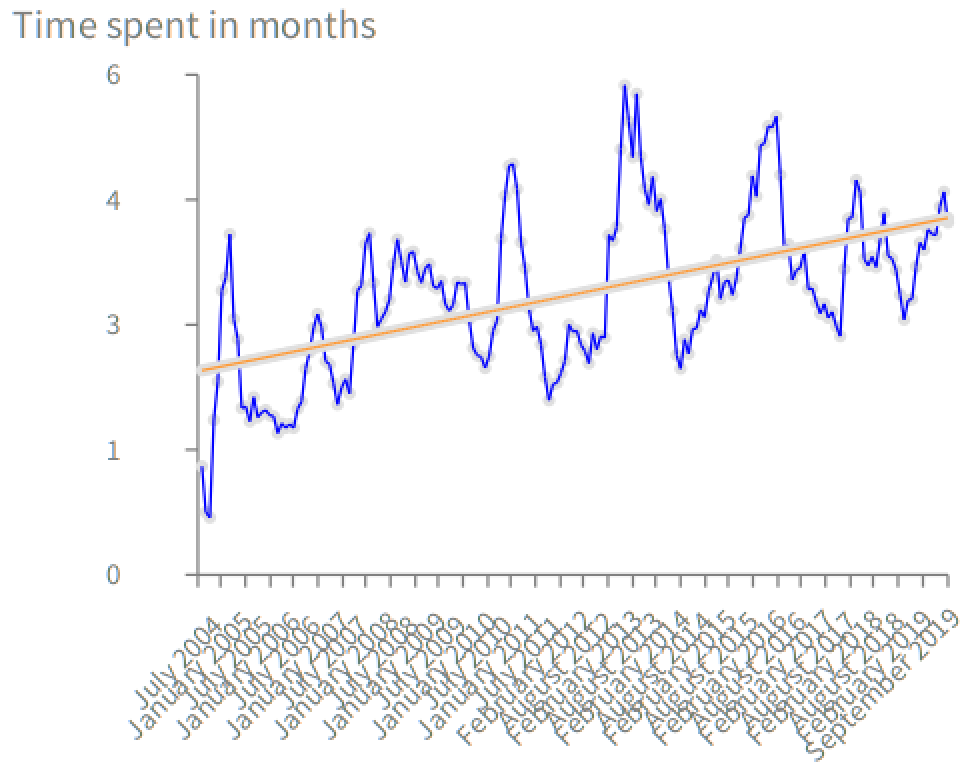
\includegraphics[width=70mm]{./images/openCloseEvol.png} \\
  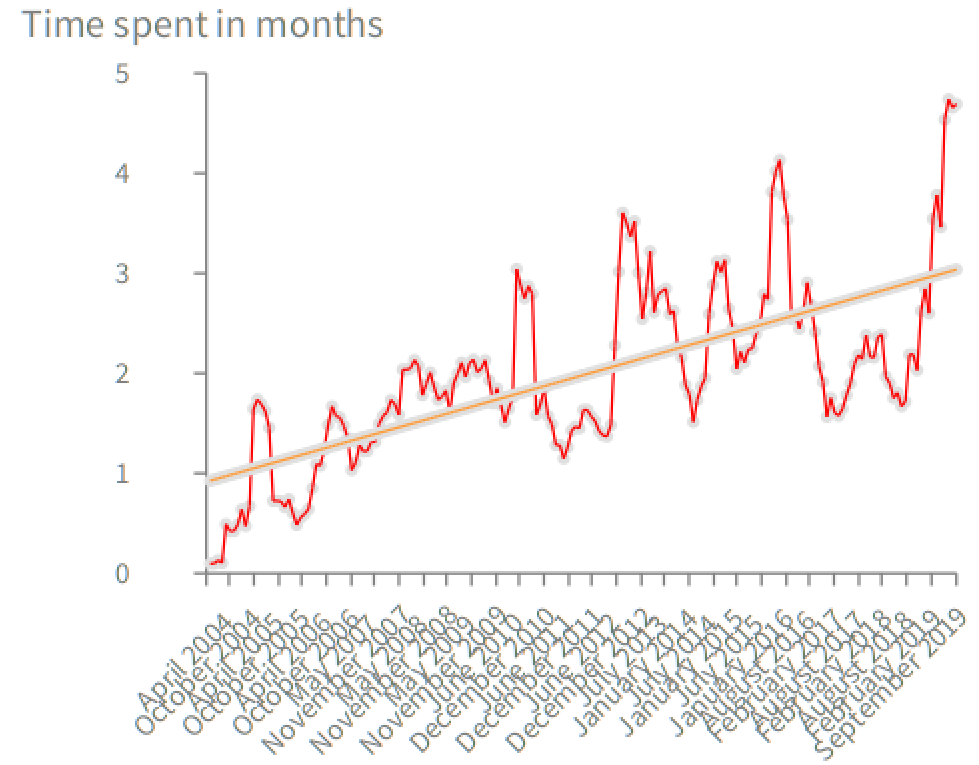
\includegraphics[width=70mm]{./images/openCloseBug.png}
  \caption{Time to close evolution (up) and defect (down) tickets}
  \label{fig:closingTime}
\end{figure}

Figure \ref{fig:closingTime} presents the trend of closing time for evolution (up) and defect (down) tickets.
One can notice a large variation of plotted time, even after smoothing it with the moving average.


It takes longer (on average) to close an evolution ticket than a defect ticket which seems natural.

We also note that the time is augmenting over the years for both categories which may be a sign of declining quality.
Finally we note that the closing time over the 15 years was multiplied by 2 for evolution tickets and 3 for defect tickets.
Again this is an issue to investigate.


\subsubsection{Developer time spent on a ticket}
%-------------------------------------------------------------------------------

When a developer works on a ticket, he spent time to analyze the task. 
He then implements a solution and then tests.
 The time spent analyzing and implementing solution for the ticket depends on the workload of the ticket, the complexity of the system, etc.  

\begin{figure}[htbp]
  \centering
  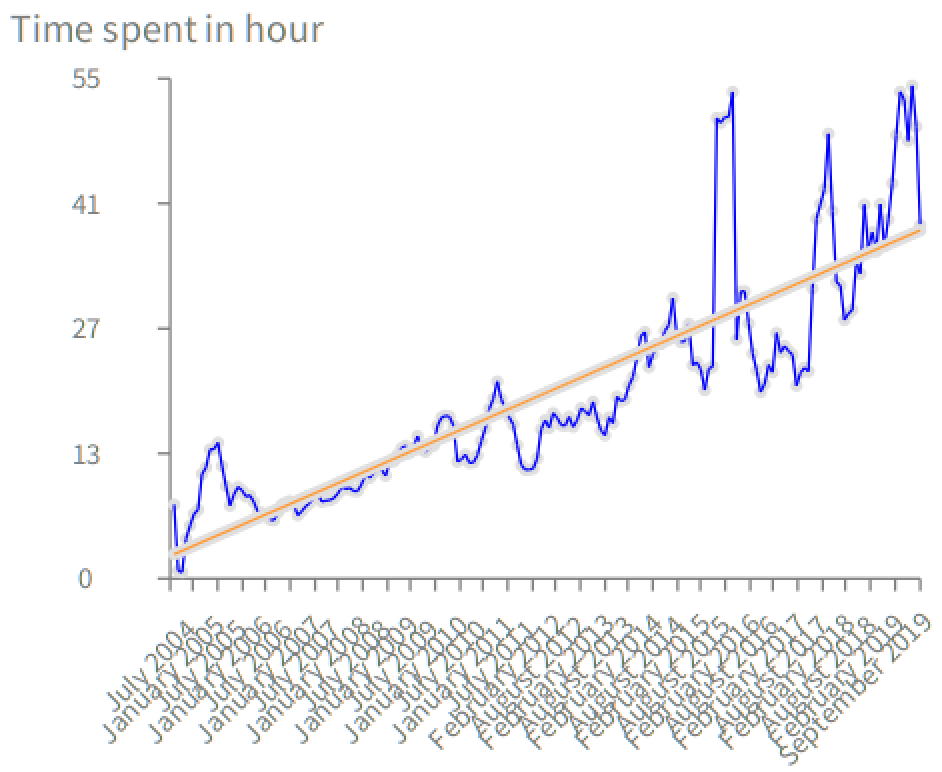
\includegraphics[width=70mm]{./images/devEvol.png}\\
  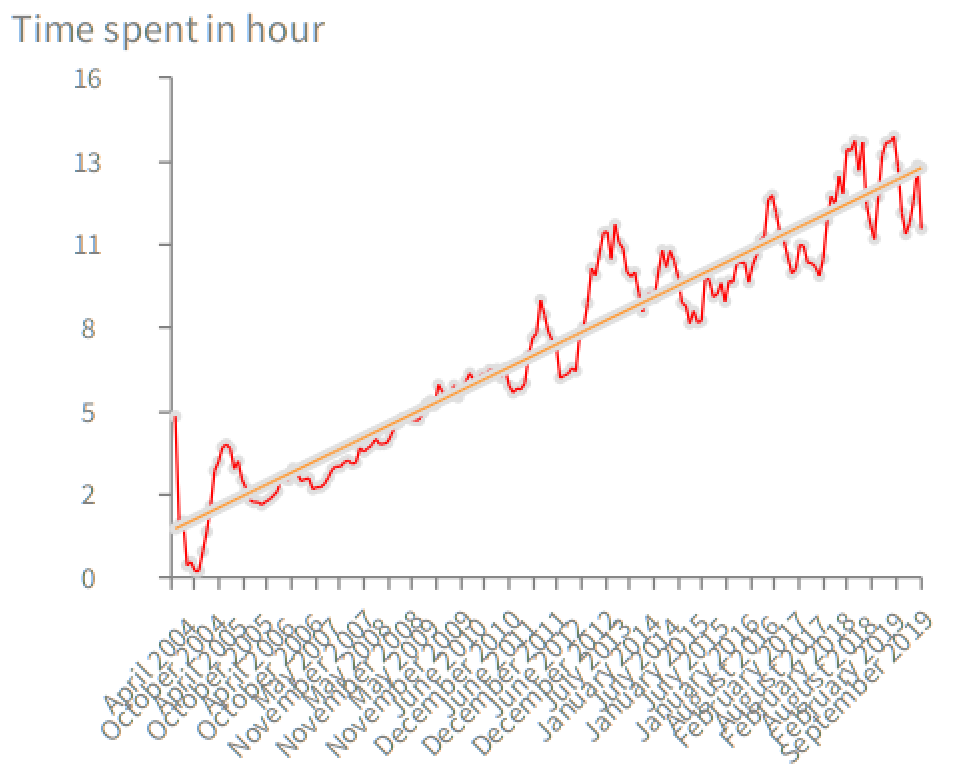
\includegraphics[width=70mm]{./images/devDefect.png}
  \caption{Time spent by a developer to implement his solution for  evolution (up) and defect (down) tickets}
  \label{fig:devTimeDev}
\end{figure}

%ressemble a closing time
Figure \ref{fig:devTimeDev} presents the trend of closing time for evolution (up) and defect (down) tickets.
One can notice a large variation of plotted time spent by the developer, even after smoothing it with the moving average.

It takes longer (on average) to implement a solution for an evolution ticket than a defect ticket which seems natural.

We also note that the time is augmenting over the years for both categories which may be a sign of declining quality.
Finally, we note that the closing time over the 15 years was multiplied by 1.5 for evolution tickets and 4 for defect tickets.
This is an issue to investigate.
\subsubsection{Time  to test a ticket after development}
%-------------------------------------------------------------------------------

% constant pour defect -> OK
% en diminution pour evolution -> peut-etre du a un manque de temps. Peut-etre cause d'une perte de quality et d' une augmentation des bugs

 \begin{figure}[htbp]
  \centering
  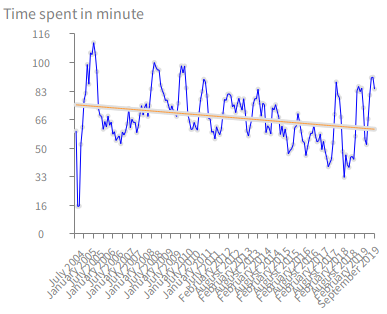
\includegraphics[width=70mm]{./images/evolutionTest.png} \\
  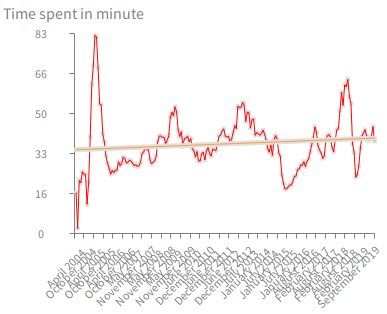
\includegraphics[width=70mm]{./images/timeDevTest.png}
  \caption{Time spent by a developer to test his solution for  evolution (up) and defect (down) tickets}
  \label{fig:devTimeTest}
\end{figure}
Figure \ref{fig:devTimeTest} presents the trend of the time spent by a developer to test his solution for evolution (up) and defect (down) tickets.
We can observe that the time spent on testing evolution tickets is decreasing. 
This might be because developers lack to test evolution tickets. The lost of quality of the system and the growing number of defects in the system may also be the reason.
The time spent to test defects tickets is relatively constant which is ok.
 
\subsubsection{Time estimation}
 %-------------------------------------------------------------------------------

%2 periodes tres claires en quelle annee et du a un effort explicite pour mieux evaluer le temps qui est maintenant fait en interne par la manager.

%avant on est audessus de 0 donc sous-estimation qui en plus est en croissance
%apres en dessous donc sur-estimationde pire en pire pour les defauts mais de moins en moins pour les evolutionos avec une moyenne proche de 0

\begin{figure}[htbp]
  \centering
  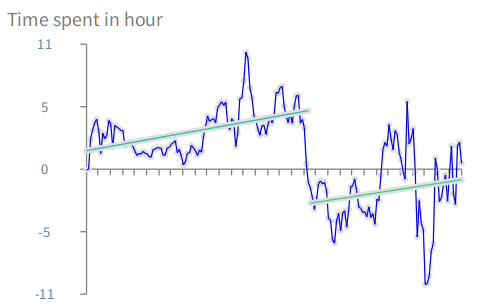
\includegraphics[width=70mm]{./images/estimateEvol.png}\\
  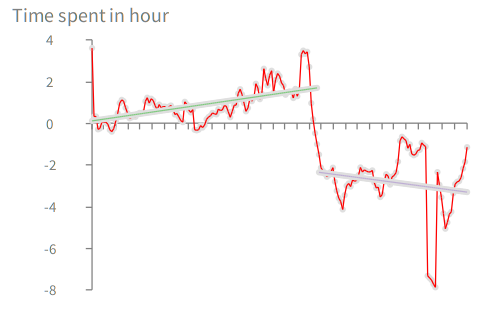
\includegraphics[width=70mm]{./images/estimateBug.png}
  %\caption{Actual time spent by the developer minus time estimated by the manager for evolution tickets. 
   % The yAxis represent the value of the gap between the development time and the estimated time in hour. 
    %The xAxis represent months from 2004 to 2019}
    \caption{Difference between time spent by a developer  and time estimated for  evolution (up) and defect (down) tickets}
  \label{fig:devEst}
\end{figure}

Figure \ref{fig:devEst} shows the trend the difference between the time spent by the developer and the time estimated for evolution (up) and defect (down) tickets.
One can notice two obvious periods. 
 A period before may 2013 the time spent by the developer is superior to the time estimated with and increasing variation for evolution and defect tickets. 
 A period after May 2013 the time estimated is superior to the time spent by the developer for evolution and defect tickets. 
 This estimate is improving for evolution tickets as the regression line is closing to 0.
But for defects tickets the overestimation trend to increase.

% \section{Discussion}
% %-------------------------------------------------------------------------------
% \label{sec:results-discussion}

% \begin{itemize}
%     \item From 2004 to 2019, as we can see in figure \ref{fig:evol} and figure \ref{fig:defect} ,  the time to close a ticket is 5 times the time at 2004 for defects and 1.5 times for evolution.
%     \item Developers spend 4 times the time spent at 2004 for evolution tickets figure \ref{fig:devTimeEvol}, and  3 times for defects tickets figure \ref{fig:devTimeDefect}.
%     \item  Figure \ref{fig:devTimeTestEvol} and \ref{fig:devTimeTestBug} show that the developer spend in average 45 minutes test  the feature implemented of the fixed defect.
%     \item The time estimated by the developers team manager trend to be enough for the developer from 2013 for defects tickets and evolutions tickets.
% \end{itemize}

\section{Summary and Conclusions}
%-------------------------------------------------------------------------------
\label{sec:conclusion}

In this paper, we present our first step in improving practices in a french company. We first introduce subversion, a version control system.
The developers' team is now using it and the software studied source code is now versioned.
This opens the door for further analysis of the code repository to understand the system evolution. 
Using the ticket database, the moving average and regression line, we build a defect model mainly assess the developer effort throughout the project life cycle. We will use this model to monitor our future actions which are: how to decompose the system big methods.
\bibliographystyle{plainnat}
%\bibliographystyle{alpha}
\bibliography{rmod,other,new}

\vspace{12pt}
\end{document}
